\section{Tiefenanpassungen durch Farbbilder}

Aus allen zuvor beschriebenen Verfahren werden letztendlich Tiefeninformationen, in Form von geometrischen Primitiven oder Punkten im Raum gewonnen. Diese werden passend zur aktuellen Kameraposition als Tiefenbild gerendert und füllen den Z-Buffer für eine entsprechende Aussparungen bei der Überdeckung virtueller Objekte. Auf Grund von Sensorungenauigkeiten und größeren Auflösungen der Rekonstruktionsverfahren können dabei fehlerhafte Tiefeninformationen im Z-Buffer gelangen, die zu Fehlern bei der Bestimmung der Überdeckung führen können. Dieses Problem ist am Beispiel der Pointcloud Projektion aus Kapitel \ref{sec:pc-projection} in Abbildung \ref{fig:pc-noise} zu erkennen. 

\begin{figure}[h]
  \centering
	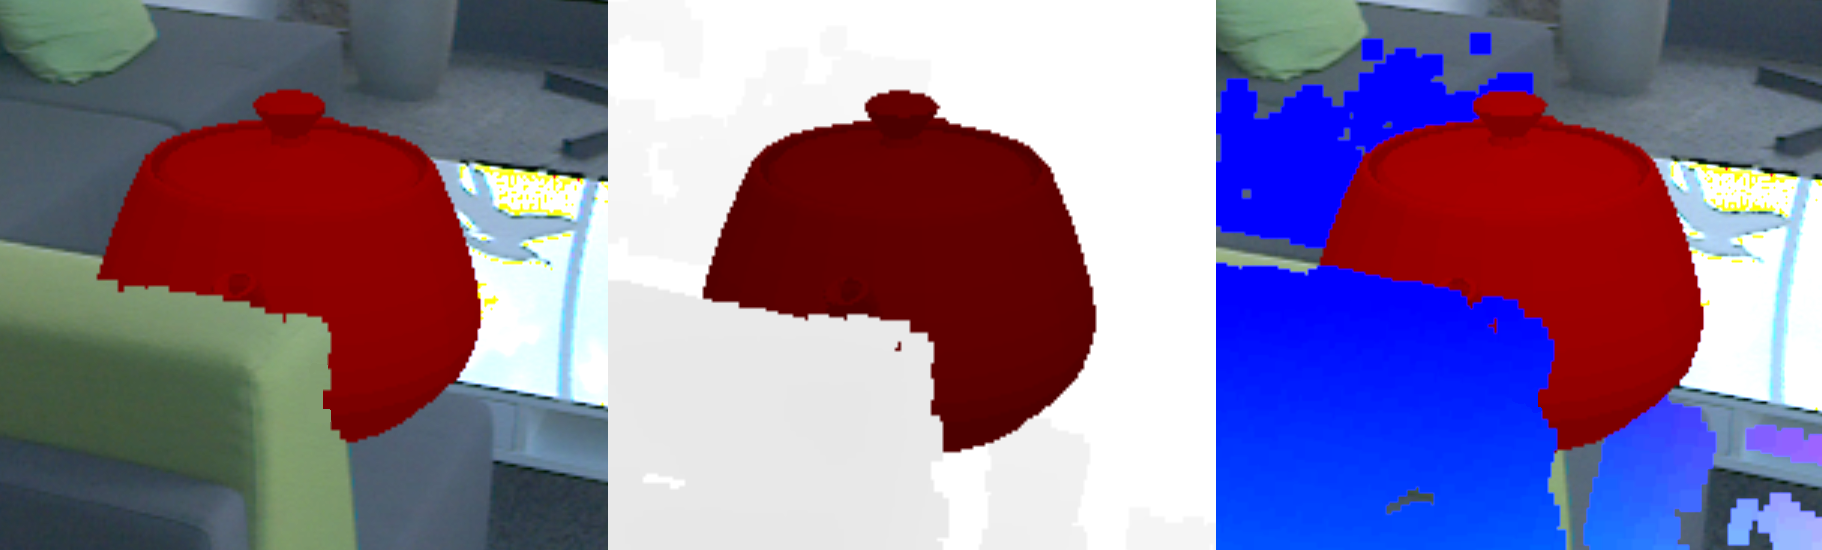
\includegraphics[width=1.0\textwidth]{content/images/methods/pc-noise.png} 
  \caption{Überdeckung mit einfacher Pointcloud Projektion. Links: Resultat der Überdeckung. Mitte: Darstellung des Tiefepuffers. Rechts: Darstellung der Pointcloud.}
  \label{fig:pc-noise}
\end{figure}

Die Reduktion von Ungenauigkeiten im Tiefenbild könnte durch einen einfachen Weichzeichner erreicht werden. Dieser würde jedoch die Kanten im Farbbild nicht berücksichtigen und somit fehlerhafte Tiefengradienten an den Kanten erzeugen und einen durchaus größeren Fehler generieren. \citet{newcombe2011kinectfusion} wenden einen sogenannten \enquote{Bilateralen Filter} in ihrem KinectFusion Rekonstruktionsverfahren an, bevor sie die Tiefeninformationen in die TSDF Repräsentation einfließen lassen. Dieser Filter von \citet{tomasi1998bilateral} ermöglicht das Weichzeichnen ohne dabei die Kanten im Bild zu übergehen, bezieht sich jedoch nur auf das selbe Bild, auf dem der Filter angewendet wird. 

\citet{liu2012guided} hingegen wenden einen sogenannten \enquote{Guided Filter} in Ihrem Verfahren zur Optimierung der der Tiefeninformationen für Kinect ähnliche Sensoren auf das Tiefenbild an. Dieser Filter von \citet{he2010guided} ist in der Lage, auf Grundlage eines anderen Leitbildes ein Weichzeichnen durchzuführen, ohne dabei die Kanten des Leitbildes zu überschreiten. Auch wenn \citet{petschnigg2004digital} eine Erweiterung, den Joint Bilateral Filter, vorstellen, der auf Basis eines anderen Leitbildes eine Weichzeichnung ohne Kantenüberschreitung ermöglicht, bietet der Guided Filter eine deutlich bessere Performance. Außerdem verhindert der Guided Filter Fehlerartefakte im Resultat, die bei dem Bilateralen Filter an den Kanten auftreten können. \citep{he2010guided} 

Ausgehend von der Eingangsgrafik \(p\), einem Leitbild \(I\) und dem Ergebnisbild \(q\) wird das grundlegende Modell dieser Art von Filter mit der Gleichung \ref{eq:gf-model} beschrieben. Diese Gleichung findet für jeden Pixel \(i\) in \(q\) eine gewichtete Summe über jeden Pixel \(j\) einer vordefinierten Ausschnittgröße. \(W_{ij}\) entspricht dabei dem Gewicht, welches für die jeweiligen Pixel \(p_j\) gilt. Bei dieser Faltung gilt üblicherweise  \(\sum_{j} W_{ij}(I)=1 \forall i \in [1\ldots |p|]\). \citep{he2010guided}

\begin{equation} \label{eq:gf-model}
q_{i} = \sum_j W_{ij}(I)p_j
\end{equation}

Der Filterkern \(W_{ij}(I)\) vom Guided Filter, zu finden in Gleichung \ref{eq:gf-W}, ist, wie auch beim bilateralen Filter, abhängig von einem Leitbild \(I\), um die Gewichte entsprechend den Kanten des Leitbildes an der Position ermitteln zu können. Die Variablen \(\mu_k\) und \(\sigma^2_k\) beschreiben jeweils den Mittelwert und die Abweichung des Leitbildes im Bildausschnitt \(w_k\). \(|w|\) entspricht der Pixelgröße des Ausschnitts. \citep{he2010guided}

\begin{equation} \label{eq:gf-W}
W_{ij}(I) = \frac{1}{|w|^2} \sum_{k:(i,j) \in w_k} (1+\frac{(I_i-\mu_k)(I_j-\mu_k)}{\sigma^2_k + \epsilon})
\end{equation}

Dieser Filterprozess wird auch als eine translationsabhänige Faltung bezeichnet, die üblicherweise aufwändig ist und dessen Berechnungsaufwand abhängig zur Filterkern Größe (\(|w|\)) ist. \citet{he2010guided} stellen jedoch noch eine andere Definition des Filters zur Verfügung, in denen alle Summen der Form \(\sum_i\in w_k f_i\) entsprechen und dadurch mit der Bildintegrationstechnik von \citet{crow1984summed} in \(O(N)\) gelöst werden können. Der Guided Filter wird in der letztendlichen Implementierung nach Gleichung \ref{eq:gf-final} implementiert, in der die Koeffizienten \(\overline{a}_i\) und \(\overline{b}_i\) dem Mittelwert über \(a_k\) aus Gleichung \ref{eq:gf-a} und \(b_k\) aus Gleichung \ref{eq:gf-b} für jedes Fenster \(w_k\) entspricht. So wird auch \(\overline{p}_k\) durch \(\frac{1}{|w|} \sum_{i \in w_k} p_i\) berechnet.

\begin{equation} \label{eq:gf-final}
q_i = \overline{a}_iI_i+\overline{b_i}
\end{equation}

\begin{equation} \label{eq:gf-a}
a_k = \frac{\frac{1}{w} \sum_{i \in w_k} I_i p_I - \mu_k \overline{p}_k}{\sigma_k^2+\epsilon}
\end{equation}

\begin{equation} \label{eq:gf-b}
b_k = \overline{p}_k - a_k\mu_k
\end{equation}

Der Faktor \(\epsilon\) reguliert im beschriebenen Filter von \citet{he2010guided} welcher Bildanteil als beizubehaltende Kante im resultierenden Bild gewertet werden soll und somit stärker oder schwächer in die Gewichtung \(W_{ij}\) Einfluss nimmt. Neben diesem Regulierungsfaktor ist auch die Wahl des Radius \(r\) für den Ausschnitt \(w_k\) als Eingabe für diesen Filter wichtig. Der Radius wirkt sich laut \citet{he2010guided} jedoch nicht wie beim bilateralen Filter auf die Laufzeit des Filters aus. 

\begin{quote}
\enquote{One more advantage of the guided filter over the bilateral filter is that it automatically has an \(O(N)\) time exact algorithm. \(O(N)\) time implies that the time complexity is independent of the window radius \(r\), so we are free to use arbitrary kernel sizes in the applications.} \citep{he2010guided}
\end{quote}

\begin{figure}[h]
  \centering
	
\includegraphics[width=1.0\textwidth]{content/images/methods/gf-result.png} 
  \caption{Guided Filter Anwendungsbeispiel. Das Tiefenbild links ergibt durch den Guided Filter mit dem Leitbild in der Mitte das Ergebnis im rechten Bild.}
  \label{fig:gf-result}
\end{figure}

Mit einer Komplexität von \(O(N)\) findet dieser Filter erfolgreich Anwendung in verschiedensten Bereichen. Er wird zum Beispiel zur Rauschunterdrückung, dem Weichzeichnen oder Verstärken von Details, zur HDR Kompression, dem Entfernen von matten Bildeigenschaften oder, wie in diesem Fall, zum zusammengeführten Anreichern von Bildinformationen verwendet \citep{he2010guided}. Angewendet auf das ermittelte Tiefenbild kann dieser Guided Filter, mit dem jeweiligen RGB Bild als Leitbild, ein Rauschen eliminieren und die Kanten der Tiefeninformationen durch ein entsprechend groß gewählten Fensterradius \(r\) und Regulierungsfaktors \(\epsilon\), an die Kanten der Kameraaufnahme angleichen \citep{liu2012guided}. Ein Beispiel für eine erfolgreiche Anwendung dieses Filters ist in Abbildung \ref{fig:gf-result} zu sehen.


